% PDCA cycle
% Author: tikzanfaenger, Helmut, and Bartman
\documentclass[tikz,border=10pt]{standalone}
\usetikzlibrary{decorations.text}
\definecolor{mygray}{RGB}{208,208,208}
\definecolor{mymagenta}{RGB}{226,0,116}
\newcommand*{\mytextstyle}{\sffamily\Large\bfseries\color{black!85}}
\newcommand{\arcarrow}[3]{%
   % inner radius, middle radius, outer radius, start angle,
   % end angle, tip protusion angle, options, text
   \pgfmathsetmacro{\rin}{1.7}
   \pgfmathsetmacro{\rmid}{2.2}
   \pgfmathsetmacro{\rout}{2.7}
   \pgfmathsetmacro{\astart}{#1}
   \pgfmathsetmacro{\aend}{#2}
   \pgfmathsetmacro{\atip}{5}
   \fill[mygray, very thick] (\astart+\atip:\rin)
                         arc (\astart+\atip:\aend:\rin)
      -- (\aend-\atip:\rmid)
      -- (\aend:\rout)   arc (\aend:\astart+\atip:\rout)
      -- (\astart:\rmid) -- cycle;
   \path[
      decoration = {
         text along path,
         text = {|\mytextstyle|#3},
         text align = {align = center},
         raise = -1.0ex
      },
      decorate
   ](\astart+\atip:\rmid) arc (\astart+\atip:\aend+\atip:\rmid);
}
\begin{document}
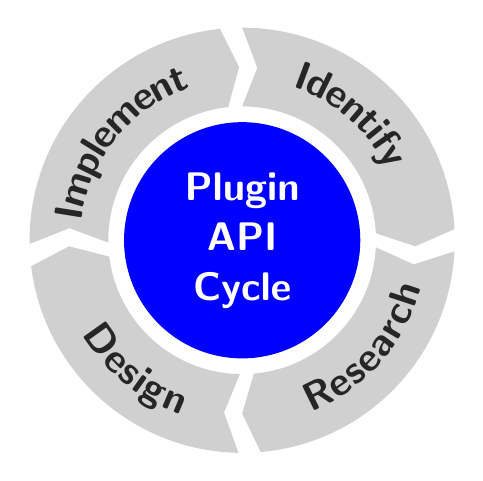
\begin{tikzpicture}
   \fill[even odd rule,blue] circle (1.5);

   \node at (0,0) [
      font  = \mytextstyle,
      color = white,
      align = center
   ]{
       Plugin \\
       API\\
      Cycle
   };
   \arcarrow{ 85}{  3}{ Identify }
   \arcarrow{270}{357}{ Research }
   \arcarrow{182}{269}{ Design }
   \arcarrow{176}{ 96}{ Implement   }
\end{tikzpicture}
\end{document}